\renewcommand{\FileName}{twobytwo}

\begin{frame}
%\makeatletter\slidebox@restore\makeatother
\frametitle{Graphical Methods for 2$\times$2 tables: Example}
\begin{itemize}
 \item \citet{Bickel-etal:75}: data on admissions to graduate departments
 at Berkeley in 1973.
 \item Aggregate data for the six largest departments:
 \begin{table}[htb]
\caption{Admissions to Berkeley graduate programs}
\label{tab:berk22}
 \begin{center}
\begin{tabular}{lrr|rrr}
\hline
  & Admitted & Rejected & Total & \red{\% Admit} & \red{Odds(Admit)}\\
\hline
 Males & 1198 & 1493 & 2691  & \red{44.52} & \red{0.802}\\
 Females & 557 & 1278 & 1835 & \red{30.35} & \red{0.437}\\
\hline
 Total & 1755 & 2771 & 4526  & 38.78 & 0.633\\
\hline
\end{tabular}
\end{center}
\end{table}


 \item Evidence for gender bias?
 \begin{itemize}

 \item Odds ratio, 
 $\theta = \frac{\mbox{Odds}(\mbox{Admit}\given\mbox{Male})}{\mbox{Odds}(\mbox{Admit}\given\mbox{Female})} = 
 \frac{1198 / 1493}{557 / 1276} = \frac{0.802}{0.437} = 
 1.84$
 \item $\rightarrow$ Males 84\% more likely to be admitted. 
 \item Chi-square tests: $G^2_{(1)} = 93.7$, $\chi^2_{(1)} = 92.2, \: p < 0.0001$
 \end{itemize}
\end{itemize}

\end{frame}
\begin{frame}[plain]
\begin{center}
\includegraphics[width=.7\textwidth]{fig/Admissions2}
\end{center}
\begin{itemize*}
 \item How to analyse these data?
 \item How to visualize \& interpret the results?
 \item Does it matter that we collapsed over Department?
\end{itemize*}


\end{frame}

\subsection{Standard analysis}
\begin{frame}[fragile]
% \makeatletter\slidebox@restore\makeatother
 \frametitle{Standard analysis: PROC FREQ}

% \vspace{2ex}
\begin{Input}
 proc freq data=berkeley;
   weight freq;
   tables gender*admit / chisq;
\end{Input}
 Output:
\begin{Output}[gobble=7,baselinestretch=.8]
               Statistics for Table of gender by admit

       Statistic                     DF       Value      Prob
       ------------------------------------------------------
       Chi-Square                     1     92.2053    <.0001
       Likelihood Ratio Chi-Square    1     93.4494    <.0001
       Continuity Adj. Chi-Square     1     91.6096    <.0001
       Mantel-Haenszel Chi-Square     1     92.1849    <.0001
       Phi Coefficient                       0.1427          
\end{Output}
 How to visualize and interpret?
\end{frame}

\subsection{Fourfold displays}
\begin{frame}
% \makeatletter\slidebox@restore\makeatother
 \frametitle{Fourfold displays for 2 $\times$ 2 tables}
 \begin{itemize*}
 \item \boldital{Quarter circles}: radius $\sim \sqrt{n_{ij}} \Rightarrow$
 \textbf{area} $\sim$ \textbf{frequency}
 \item \boldital{Independence}: Adjoining quadrants $\approx$ align
 \item \boldital{Odds ratio}: ratio of areas of diagonally opposite cells
 \item \boldital{Confidence rings}: Visual test of 
 $H_0 : \theta = 1 \leftrightarrow$ \alert{adjoining rings overlap}

 \begin{center}
   \includegraphics[width=.45\dispwidth,clip]{fig/pie2x2g}
 \end{center}
 \item Confidence rings do not overlap: $\theta \neq 1$  (reject $H_0$)
 \end{itemize*}
\end{frame}

\begin{frame}
 %\makeatletter\slidebox@restore\makeatother
 \frametitle{Fourfold displays for 2 $\times$ 2 $\times $ \textit{k} tables}
 \begin{itemize*}
 \item Data in \tabref{tab:berk22} had been pooled over departments
 \item Stratified analysis: one fourfold display for each department
 \item Each $2 \times 2$ table standardized to equate marginal frequencies
 \item Shading: highlight departments for which $H_a : \theta_i \ne 1$

 \begin{center}
 %  \includegraphics[width=.6\dispwidth,clip]{fig/pie2x2bb.eps}
   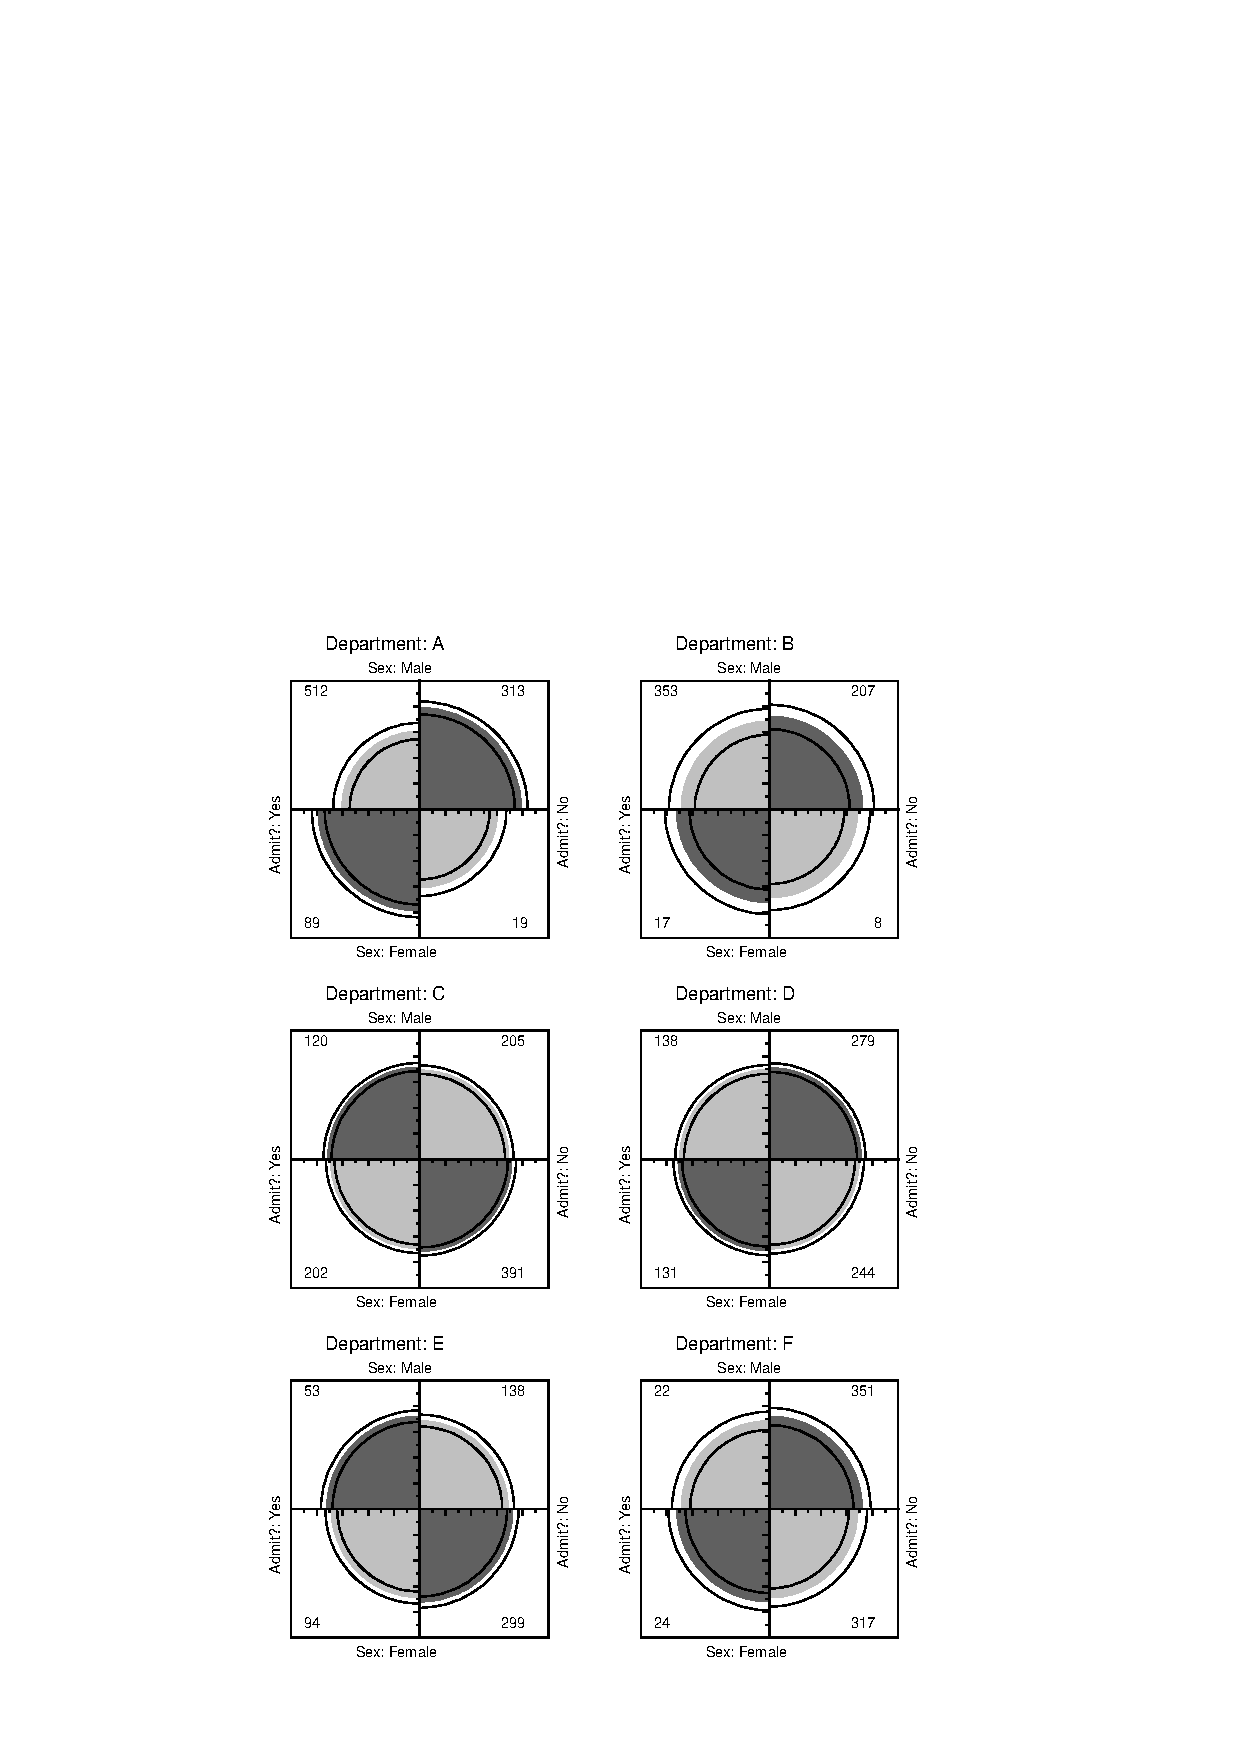
\includegraphics[width=.6\dispwidth,clip]{fig/pie2x2b}
 \end{center}
 \item Only one department (A) shows association; $\theta_A = 0.349 \rightarrow
 $ women $(0.349)^{-1} = 2.86$ times as likely as men to be admitted.
 \end{itemize*}
 \end{frame}

\begin{frame}
 %\makeatletter\slidebox@restore\makeatother
   \frametitle{What happened here?}
  Why do the results \emph{collapsed over} department disagree with the results \emph{by} department?
  \begin{block}{Simpson's paradox}
   \begin{itemize}
	 \item<1-> Aggregate data are misleading because they falsely
	 assume men and women apply \emph{equally} in each field.
	 \item<2-> But:
	   \begin{itemize*}
	   \item Large differences in admission rates across departments.
	   \item Men and women apply to these departments differentially.
	   \item Women applied in large numbers to departments with low admission rates.
	 \end{itemize*}
	 \item<3->
	  Other graphical methods can show these effects.
 	 \item<3-> (This ignores possibility of \emph{structural bias} against women:
	 differential funding of fields to which women are more likely to apply.)
  \end{itemize}
  \end{block}
\end{frame}

\begin{frame}[fragile]
%\makeatletter\slidebox@restore\makeatother

\frametitle{The \sasprogt{FOURFOLD} and the \macrot{FFOLD}}
  \begin{itemize*}
  \item The \sasprog{FOURFOLD} is written in \IML.
  \item The \macro{FFOLD} provides a simpler interface.
  \item Printed output: (a) significance tests for individual odds ratios,
  (b) tests of homogeneity of association (here, over departments) and
  (c) conditional association (controlling for department).
  \end{itemize*}
Plot by department:
\begin{Input}[fontsize=\small,label=\fbox{\texttt{berk4f.sas}},baselinestretch=0.8]
%include catdata(berkeley);

%ffold(data=berkeley, 
   var=Admit Gender,       \sascomment{/* panel variables   */} 
   \sasemph{by=Dept},                \sascomment{/* stratify by dept  */}
   down=2, across=3,       \sascomment{/* panel arrangement */}
   htext=2);               \sascomment{/* font size         */}
\end{Input}
Aggregate data: first sum over departments,
using the \macro{TABLE}:
\begin{Input}[fontsize=\small,baselinestretch=0.9,firstnumber=8]
%table(data=berkeley, \sasemph{out=berk2}, 
   var=Admit Gender,       \sascomment{/* omit dept          */}
   weight=count,           \sascomment{/* frequency variable */}
   order=data);
%ffold(\sasemph{data=berk2}, var=Admit Gender);
\end{Input}
\end{frame}

\subsection{Odds ratio plots}
\begin{frame}[fragile]
\frametitle{Odds ratio plots}
\begin{Rin}
> library(vcd)
> oddsratio(UCBAdmissions, log=FALSE)
\end{Rin}
\begin{Rout}
    A     B     C     D     E     F 
0.349 0.803 1.133 0.921 1.222 0.828 
\end{Rout}
\begin{Rin}
> lor <- oddsratio(UCBAdmissions)  # capture log odds ratios
> plot(lor)
\end{Rin}
\begin{center}
   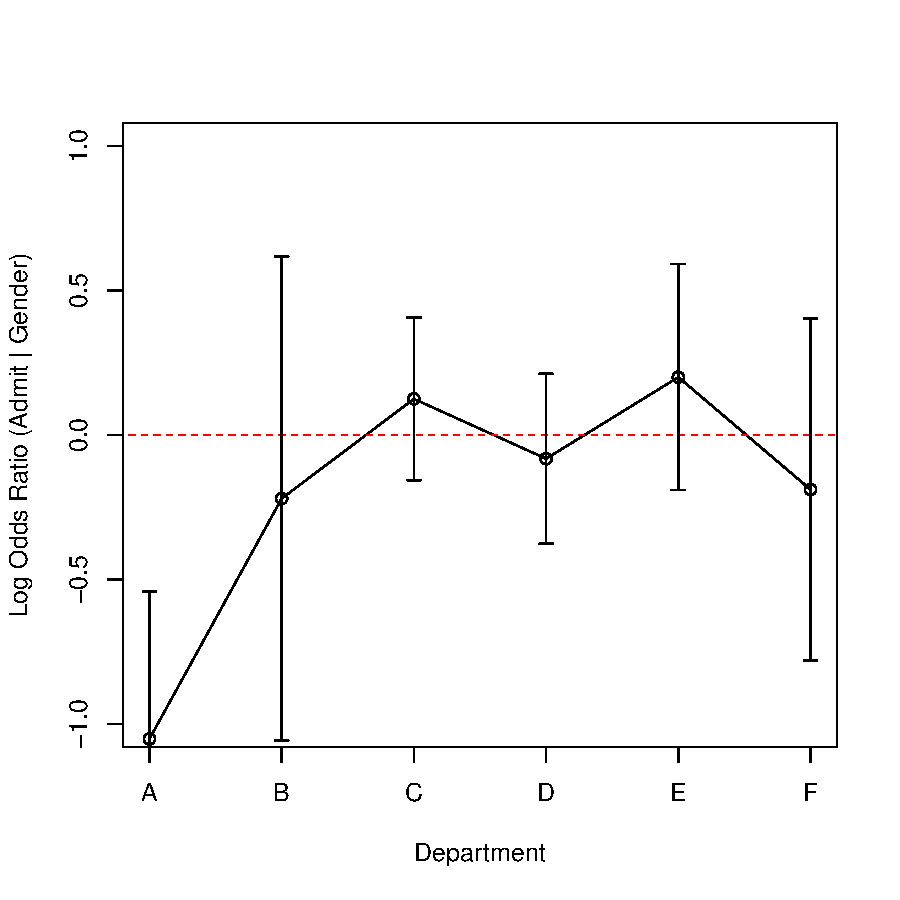
\includegraphics[width=.45\dispwidth,clip,trim=0 20 20 40]{fig/vcd-tut-oddsratio}
\end{center}

\end{frame}
